\documentclass[11pt, a4paper]{article}
\usepackage{times}
\usepackage[left=2cm, text={17cm, 24cm}, top=3cm]{geometry}
\usepackage[utf8]{inputenc}
\usepackage[czech]{babel}
\usepackage{multirow}
\usepackage[noline, czech, ruled, longend]{algorithm2e}
\usepackage{algorithmic}
\usepackage{amsmath}
\usepackage{amsthm}
\usepackage{graphicx}
\usepackage{lscape}
%
\renewcommand{\algorithmicrequire}{\textbf{Input:}}
\renewcommand{\algorithmicensure}{\textbf{Output:}}
%
\begin{document}
%
\begin{titlepage}
%
\begin{center}
%
\Huge
\textsc{Vysoké učení technické v Brně\\
\huge Fakulta informačních technologií\\}
%
\vspace{\stretch{0.382}}
%
{\LARGE
Typografie a publikování -- 3. projekt\\
\Huge Tabulky a obrázky\\}
%
\vspace{\stretch{0.618}}
%
\end{center}
{\Large \today \hfill Dominik Křivohlávek}
\medskip
\end{titlepage}
%
\section{Úvodní strana}
Název práce umístěte do zlatého řezu a nezapomeňte uvést dnešní datum a vaše jméno a příjmení.\par
%
\section{Tabulky}
Pro sázení tabulek můžeme použít buď prostředí\texttt{ tabbing }nebo prostředí\texttt{ tabular }\par
%
\subsection{Prostředí\texttt{ tabbing }}
Při použití\texttt{ tabbing }vypadá tabulka následovně:
%
\begin{tabbing}
Vodní melouny \quad\= \textbf{Cena} \quad\= \textbf{Množství} \kill
\textbf{Ovoce} \> \textbf{Cena} \> \textbf{Množství} \\
Jablka \> 25,90 \> 3 kg \\
Hrušky \> 27,40 \> 2,5 kg \\
Vodní melouny \> 35,-- \> 1 kus\\
\end{tabbing}
%
Toto prostředí se dá také použít pro sázení algoritmů, ovšem vhodnější je použít prostředí\texttt{ algorithm }nebo\texttt{ algorithm2e }(viz sekce \ref{alg}).
%
\subsection{Prostředí\texttt{ tabular }}
Další možností, jak vytvořit tabulku, je použít prostředí\texttt{ tabular}. Tabulky pak budou vypadat takto\footnote{Kdyby byl problém s\texttt{ cline, }zkuste se podívat třeba sem: {http://www.abclinuxu.cz/tex/poradna/show/325037}.}:\\
%
\begin{table}[ht]
\catcode`\-=12
\begin{center}
\begin{tabular}{|c|r|r|}
\hline
 & \multicolumn{2}{c|}{\textbf{Cena}} \\
\cline{2-3}
\textbf{Měna} & \textbf{nákup} & \textbf{prodej}\\
\hline
EUR & 27,02 &27,20\\
GBP & 31,08 & 31.80\\
USD & 25,15 & 25,51\\
\hline
\end{tabular}
\caption{Tabulka kurzů k dnešnímu dni} \label{tab1}
\end{center}
\end{table}
%
\begin{table}[ht]
\catcode`\-=12
\begin{center}
\begin{tabular}{|c|c|}
\hline
$A$ & $\neg A$\\
\hline
\textbf{P} & N\\
\hline
\textbf{O} & O\\
\hline
\textbf{X} & X\\
\hline
\textbf{N} & P\\
\hline
\end{tabular}
%
\begin{tabular}{|c|c|c|c|c|c|}
\hline
\multicolumn{2}{|c|}{\multirow{2}{*}{$A \land B$}} & \multicolumn{4}{c|}{$B$} \\ \cline{3-6} 
\multicolumn{2}{|c|}{} & \textbf{P} & \textbf{O} & \textbf{X} & \textbf{N} \\ \hline
\multirow{4}{*}{$A$} & \textbf{P} & P & O & X & N \\ \cline{2-6} 
 & \textbf{O} & O & O & N & N \\ \cline{2-6} 
 & \textbf{X} & X & N & X & N \\ \cline{2-6} 
 & \textbf{N} & N & N & N & N \\ \hline
\end{tabular}
%
\begin{tabular}{|c|c|c|c|c|c|}
\hline
\multicolumn{2}{|c|}{\multirow{2}{*}{$A \lor B$}} & \multicolumn{4}{c|}{$B$} \\ \cline{3-6} 
\multicolumn{2}{|c|}{} & \textbf{P} & \textbf{O} & \textbf{X} & \textbf{N} \\ \hline
\multirow{4}{*}{$A$} & \textbf{P} & P & P & P & P \\ \cline{2-6} 
 & \textbf{O} & P & O & P & O \\ \cline{2-6} 
 & \textbf{X} & P & P & X & X \\ \cline{2-6} 
 & \textbf{N} & P & O & X & N \\ \hline
\end{tabular}
%
\begin{tabular}{|c|c|c|c|c|c|}
\hline
\multicolumn{2}{|c|}{\multirow{2}{*}{$A \to B$}} & \multicolumn{4}{c|}{$B$} \\ \cline{3-6} 
\multicolumn{2}{|c|}{} & \textbf{P} & \textbf{O} & \textbf{X} & \textbf{N} \\ \hline
\multirow{4}{*}{$A$} & \textbf{P} & P & O & X & N \\ \cline{2-6} 
 & \textbf{O} & P & O & P & O \\ \cline{2-6} 
 & \textbf{X} & P & P & X & X \\ \cline{2-6} 
 & \textbf{N} & P & P & P & P \\ \hline
\end{tabular}
%
\caption{Protože Kleeneho trojhodnotová logika už je \uv{zastaralá}, uvádíme si zde příklad čtyřhodnotové logiky} \label{tab2}
\end{center}
\end{table}
%
\pagebreak
%
\section{Algoritmy}
\label{alg}
Pokud budeme chtít vysázet algoritmus, můžeme použít prostředí\texttt{ algorithm\footnote{Pro nápovědu, jak zacházet s prostředím\texttt{ algorithm, } můžeme zkusit tuhle stránku:\\ http://ftp.cstug.cz/pub/tex/CTAN/macros/latex/contrib/algorithms/algorithms.pdf.} }nebo\texttt{ algorithm2e\footnote{Pro\texttt{ algorithm2e }zase tuhle: http://ftp.cstug.cz/pub/tex/CTAN/macros/latex/contrib/algorithm2e/doc/algorithm2e.pdf.}}.\linebreak
Příklad použití prostředí\texttt{ algorithm2e }viz Algoritmus \ref{alg1}.\\
%
\algsetup{indent=2em}
\begin{algorithm}
\caption{\textsc{Fast}SLAM}
\label{alg1}
\SetInd{1em}{1em}
\SetNlSkip{-1.33em}
\begin{algorithmic}[1]
\REQUIRE $(X_{t-1},u_t,z_t)$
\ENSURE $X_t$
\BlankLine
\STATE $\overline{X_t} = X_t = 0$
\FOR{$k = 1$ to $M$}
\STATE $x_{t}^{[k]} =$ \emph{sample\_motion\_model}$(u_t,x_{t-1}^{[k]})$
\STATE $\omega_{t}^{[k]} =$ \emph{measurement\_model}$(z_t,x_{t}^{[k]},m_{t-1})$
\STATE $m_{t}^{[k]} = updated\_occupancy\_grid(z_t,x_{t}^{[k]},m_{t-1}^{[k]})$
\STATE $\overline{X_t} = \overline{X_t}+\langle x_{x}^{[m]}, \omega_{t}^{[m]}\rangle$
\ENDFOR
\FOR{$k = 1$ to $M$}
\STATE draw $i$ with probability $\approx \omega_{t}^{[i]}$
\STATE add $\langle x_{x}^{[k]},m_{t}^{[k]} \rangle$ to $X_t$
\ENDFOR
\RETURN $X_t$
\end{algorithmic}
\end{algorithm}
%
\section{Obrázky}
Do našich článků můžeme samozřejmě vkládat obrázky. Pokud je obrázkem fotografie, můžeme klidně použít bitmapový soubor. Pokud by to ale mělo být nějaké schéma nebo něco podobného, je dobrým zvykem takovýto obrázek vytvořit vektorově.
%
\begin{figure}[h]
\begin{center}
\scalebox{0.4}{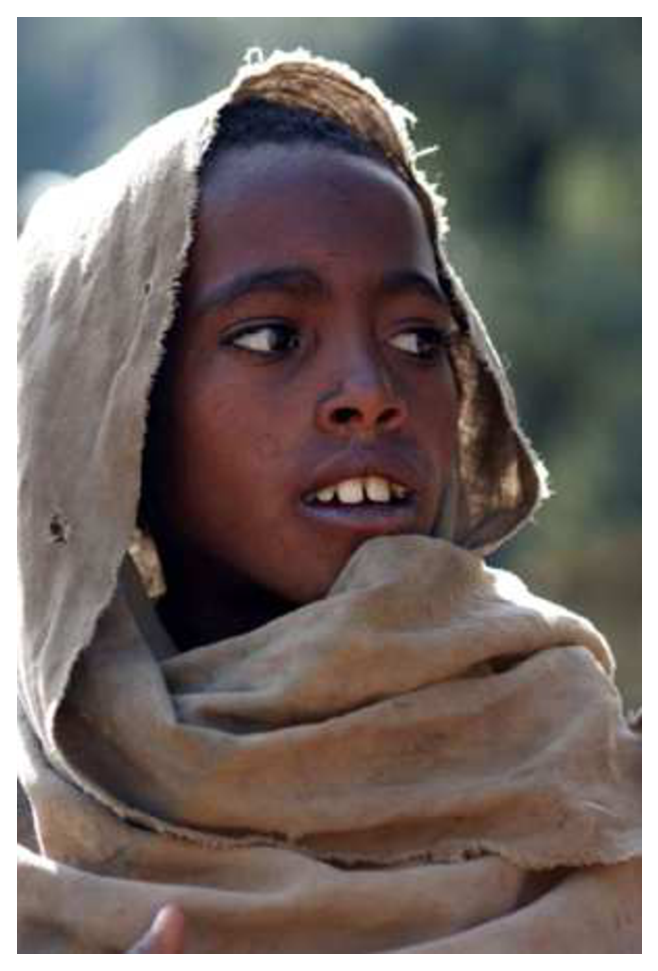
\includegraphics{etiopan.eps}\reflectbox{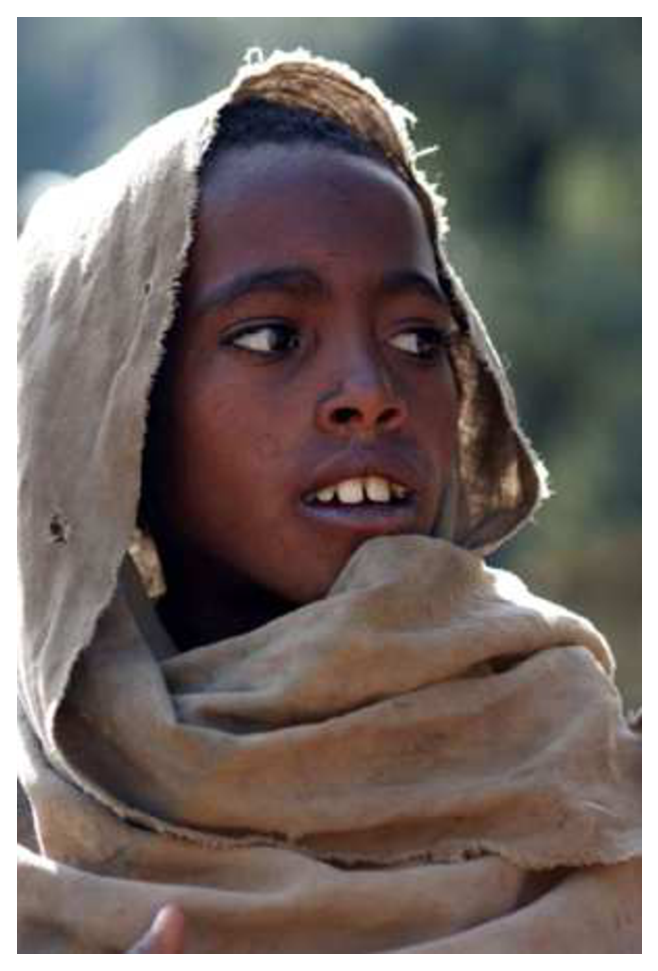
\includegraphics{etiopan.eps}}}
\caption{Malý Etiopánek a jeho bratříček} \label{obr1}
\end{center}
\end{figure}
\pagebreak\\
%
\indent Rozdíl mezi vektorovým\, \dots
%
\begin{figure}[h]
\begin{center}
\scalebox{0.4}{
\includegraphics{oniisan.eps}}
\caption{Vektorový obrázek} \label{obr2}
\end{center}
\end{figure}\\
%
\dots\,a bitmapovým obrázkem
%
\begin{figure}[h]
\begin{center}
\scalebox{0.6}{
\includegraphics{oniisan2.eps}}
\caption{Bitmapový obrázek} \label{obr3}
\end{center}
\end{figure}\\
%
se projeví například při zvětšení.\par
%
Odkazy (nejen ty) na obrázky \ref{obr1}, \ref{obr2} a \ref{obr3}, na tabulky \ref{tab1} a \ref{tab2} a také na algoritmus \ref{alg1} jsou udělány pomocí křížových odkazů. Pak je ovšem potřeba zdrojový soubor přeložit dvakrát.\par
%
Vektorové obrázky lze vytvořit i přímo v \LaTeX u, například pomocí prostředí\texttt{ picture}.
%
\newpage
\begin{landscape}
\begin{figure}
\begin{center}
\setlength{\unitlength}{4pt}
\begin{picture}(142,45)(0,0)
% hranice
\linethickness{1pt}
\put(0,0){\line(1,0){142}}
\put(0,0){\line(0,1){71}}
\put(0,71){\line(1,0){142}}
\put(142,0){\line(0,1){71}}
% tlusta cara
\linethickness{3,8pt}
\put(3,10){\line(1,0){135}}
%
\linethickness{2pt}
% prvni vertikalni OK
\put(17,10){\line(0,1){25}}
%
\linethickness{1.5pt}
% druha vertikalni
\put(25,10){\line(0,1){10}}
% treti vertikalni OK
\put(30,28){\line(0,1){4}}
% ctvrta vertikalni OK
\put(47,32){\line(0,1){7}}
% pata vertikalni
\put(53,26.25){\line(0,-1){6.75}}
%
\linethickness{1pt}
% sesta vertikalni OK
\put(87,32){\line(0,1){7}}
% sedma vertikalni OK
\put(122,32){\line(0,1){1.5}}
% osma vertikalni OK
\put(127.5,16.5){\line(0,1){10}}
% devata nahore vertikalni OK
\put(129,28){\line(0,1){4}}
% devata dole vertikalni OK
\put(129,10){\line(0,1){6.5}}
% prvni horizontalni OK
\put(62.5,16.5){\line(1,0){66.5}}
% druha horizontalni OK
\put(25,20){\line(1,0){26.5}}
% treti horizontalni
\put(53,26.5){\line(1,0){74.5}}
% ctvrta horizontalni OK
\put(30,28){\line(1,0){99}}
% pata horizontalni OK
\put(30,32){\line(1,0){99}}
% sesta horizontalni OK
\put(87,33.5){\line(1,0){35}}
% sedma horizontalni OK
\put(17,35){\line(1,0){30}}
% osma horizontalni OK
\put(47,39){\line(1,0){40}}
% prvni sikma OK
\put(30,28){\line(1,-1){8}}
% druha sikma OK
\put(51.5,20){\line(3,-1){30}}
% kruh
\linethickness{0.5pt}
\put(121,56){\circle{12}}
%
\end{picture}
\caption{Vektorový obrázek.}
\end{center}
\end{figure}
\end{landscape}
\end{document}